% Options for packages loaded elsewhere
\PassOptionsToPackage{unicode}{hyperref}
\PassOptionsToPackage{hyphens}{url}
%
\documentclass[
]{article}
\usepackage{amsmath,amssymb}
\usepackage{iftex}
\ifPDFTeX
  \usepackage[T1]{fontenc}
  \usepackage[utf8]{inputenc}
  \usepackage{textcomp} % provide euro and other symbols
\else % if luatex or xetex
  \usepackage{unicode-math} % this also loads fontspec
  \defaultfontfeatures{Scale=MatchLowercase}
  \defaultfontfeatures[\rmfamily]{Ligatures=TeX,Scale=1}
\fi
\usepackage{lmodern}
\ifPDFTeX\else
  % xetex/luatex font selection
\fi
% Use upquote if available, for straight quotes in verbatim environments
\IfFileExists{upquote.sty}{\usepackage{upquote}}{}
\IfFileExists{microtype.sty}{% use microtype if available
  \usepackage[]{microtype}
  \UseMicrotypeSet[protrusion]{basicmath} % disable protrusion for tt fonts
}{}
\makeatletter
\@ifundefined{KOMAClassName}{% if non-KOMA class
  \IfFileExists{parskip.sty}{%
    \usepackage{parskip}
  }{% else
    \setlength{\parindent}{0pt}
    \setlength{\parskip}{6pt plus 2pt minus 1pt}}
}{% if KOMA class
  \KOMAoptions{parskip=half}}
\makeatother
\usepackage{xcolor}
\usepackage[margin=1in]{geometry}
\usepackage{color}
\usepackage{fancyvrb}
\newcommand{\VerbBar}{|}
\newcommand{\VERB}{\Verb[commandchars=\\\{\}]}
\DefineVerbatimEnvironment{Highlighting}{Verbatim}{commandchars=\\\{\}}
% Add ',fontsize=\small' for more characters per line
\usepackage{framed}
\definecolor{shadecolor}{RGB}{248,248,248}
\newenvironment{Shaded}{\begin{snugshade}}{\end{snugshade}}
\newcommand{\AlertTok}[1]{\textcolor[rgb]{0.94,0.16,0.16}{#1}}
\newcommand{\AnnotationTok}[1]{\textcolor[rgb]{0.56,0.35,0.01}{\textbf{\textit{#1}}}}
\newcommand{\AttributeTok}[1]{\textcolor[rgb]{0.13,0.29,0.53}{#1}}
\newcommand{\BaseNTok}[1]{\textcolor[rgb]{0.00,0.00,0.81}{#1}}
\newcommand{\BuiltInTok}[1]{#1}
\newcommand{\CharTok}[1]{\textcolor[rgb]{0.31,0.60,0.02}{#1}}
\newcommand{\CommentTok}[1]{\textcolor[rgb]{0.56,0.35,0.01}{\textit{#1}}}
\newcommand{\CommentVarTok}[1]{\textcolor[rgb]{0.56,0.35,0.01}{\textbf{\textit{#1}}}}
\newcommand{\ConstantTok}[1]{\textcolor[rgb]{0.56,0.35,0.01}{#1}}
\newcommand{\ControlFlowTok}[1]{\textcolor[rgb]{0.13,0.29,0.53}{\textbf{#1}}}
\newcommand{\DataTypeTok}[1]{\textcolor[rgb]{0.13,0.29,0.53}{#1}}
\newcommand{\DecValTok}[1]{\textcolor[rgb]{0.00,0.00,0.81}{#1}}
\newcommand{\DocumentationTok}[1]{\textcolor[rgb]{0.56,0.35,0.01}{\textbf{\textit{#1}}}}
\newcommand{\ErrorTok}[1]{\textcolor[rgb]{0.64,0.00,0.00}{\textbf{#1}}}
\newcommand{\ExtensionTok}[1]{#1}
\newcommand{\FloatTok}[1]{\textcolor[rgb]{0.00,0.00,0.81}{#1}}
\newcommand{\FunctionTok}[1]{\textcolor[rgb]{0.13,0.29,0.53}{\textbf{#1}}}
\newcommand{\ImportTok}[1]{#1}
\newcommand{\InformationTok}[1]{\textcolor[rgb]{0.56,0.35,0.01}{\textbf{\textit{#1}}}}
\newcommand{\KeywordTok}[1]{\textcolor[rgb]{0.13,0.29,0.53}{\textbf{#1}}}
\newcommand{\NormalTok}[1]{#1}
\newcommand{\OperatorTok}[1]{\textcolor[rgb]{0.81,0.36,0.00}{\textbf{#1}}}
\newcommand{\OtherTok}[1]{\textcolor[rgb]{0.56,0.35,0.01}{#1}}
\newcommand{\PreprocessorTok}[1]{\textcolor[rgb]{0.56,0.35,0.01}{\textit{#1}}}
\newcommand{\RegionMarkerTok}[1]{#1}
\newcommand{\SpecialCharTok}[1]{\textcolor[rgb]{0.81,0.36,0.00}{\textbf{#1}}}
\newcommand{\SpecialStringTok}[1]{\textcolor[rgb]{0.31,0.60,0.02}{#1}}
\newcommand{\StringTok}[1]{\textcolor[rgb]{0.31,0.60,0.02}{#1}}
\newcommand{\VariableTok}[1]{\textcolor[rgb]{0.00,0.00,0.00}{#1}}
\newcommand{\VerbatimStringTok}[1]{\textcolor[rgb]{0.31,0.60,0.02}{#1}}
\newcommand{\WarningTok}[1]{\textcolor[rgb]{0.56,0.35,0.01}{\textbf{\textit{#1}}}}
\usepackage{graphicx}
\makeatletter
\def\maxwidth{\ifdim\Gin@nat@width>\linewidth\linewidth\else\Gin@nat@width\fi}
\def\maxheight{\ifdim\Gin@nat@height>\textheight\textheight\else\Gin@nat@height\fi}
\makeatother
% Scale images if necessary, so that they will not overflow the page
% margins by default, and it is still possible to overwrite the defaults
% using explicit options in \includegraphics[width, height, ...]{}
\setkeys{Gin}{width=\maxwidth,height=\maxheight,keepaspectratio}
% Set default figure placement to htbp
\makeatletter
\def\fps@figure{htbp}
\makeatother
\setlength{\emergencystretch}{3em} % prevent overfull lines
\providecommand{\tightlist}{%
  \setlength{\itemsep}{0pt}\setlength{\parskip}{0pt}}
\setcounter{secnumdepth}{-\maxdimen} % remove section numbering
\usepackage{booktabs}
\usepackage{longtable}
\usepackage{array}
\usepackage{multirow}
\usepackage{wrapfig}
\usepackage{float}
\usepackage{colortbl}
\usepackage{pdflscape}
\usepackage{tabu}
\usepackage{threeparttable}
\usepackage{threeparttablex}
\usepackage[normalem]{ulem}
\usepackage{makecell}
\usepackage{xcolor}
\ifLuaTeX
  \usepackage{selnolig}  % disable illegal ligatures
\fi
\IfFileExists{bookmark.sty}{\usepackage{bookmark}}{\usepackage{hyperref}}
\IfFileExists{xurl.sty}{\usepackage{xurl}}{} % add URL line breaks if available
\urlstyle{same}
\hypersetup{
  pdftitle={Child Marriage Phenomenon In Vietnam},
  pdfauthor={Holly Duong},
  hidelinks,
  pdfcreator={LaTeX via pandoc}}

\title{Child Marriage Phenomenon In Vietnam}
\author{Holly Duong}
\date{2024-02-29}

\begin{document}
\maketitle

\begin{Shaded}
\begin{Highlighting}[]
\CommentTok{\# load packages}
\FunctionTok{library}\NormalTok{(readr)}
\FunctionTok{library}\NormalTok{(dplyr)}
\FunctionTok{library}\NormalTok{(ggplot2)}
\FunctionTok{library}\NormalTok{(gridExtra)}
\FunctionTok{library}\NormalTok{(corrplot)}
\FunctionTok{library}\NormalTok{(plotly)}
\FunctionTok{library}\NormalTok{(reshape2)}
\FunctionTok{library}\NormalTok{(car)}
\FunctionTok{library}\NormalTok{(kableExtra)}
\FunctionTok{library}\NormalTok{(broom)}
\FunctionTok{library}\NormalTok{(knitr)}
\FunctionTok{library}\NormalTok{(pROC)}
\FunctionTok{library}\NormalTok{(ggpattern)}
\FunctionTok{library}\NormalTok{(tidyr)}
\end{Highlighting}
\end{Shaded}

\hypertarget{setting-up-data}{%
\subsubsection{Setting up Data}\label{setting-up-data}}

\begin{Shaded}
\begin{Highlighting}[]
\CommentTok{\# import dataset}
\NormalTok{female }\OtherTok{\textless{}{-}} \FunctionTok{read\_csv}\NormalTok{(}\StringTok{"/Users/hollyduong/Desktop/DA 401/ChildMarriageInVietnam/Data/wm.csv"}\NormalTok{)}
\end{Highlighting}
\end{Shaded}

\begin{Shaded}
\begin{Highlighting}[]
\CommentTok{\# get a glimpse of dataset}
\FunctionTok{head}\NormalTok{(female)}
\end{Highlighting}
\end{Shaded}

\begin{verbatim}
## # A tibble: 6 x 458
##     HH1   HH2    LN   WM1   WM2   WM3 WMINT   WM4   WM5  WM6D  WM6M  WM6Y   WM8
##   <dbl> <dbl> <dbl> <dbl> <dbl> <dbl> <dbl> <dbl> <dbl> <dbl> <dbl> <dbl> <dbl>
## 1     1     2     3     1     2     3    92    91    92    19    11  2020     2
## 2     1     4     2     1     4     2    92    91    92    18    11  2020     1
## 3     1     9     4     1     9     4    92    91    92    18    11  2020     1
## 4     1    10     4     1    10     4    92    91    92    18    11  2020     2
## 5     1    11     4     1    11     4    92    91    92    19    11  2020     2
## 6     1    11     5     1    11     5    92    91    92    18    11  2020     2
## # i 445 more variables: WM9 <dbl>, WM17 <dbl>, WM7H <dbl>, WM7M <dbl>,
## #   WM10H <dbl>, WM10M <dbl>, WM11 <dbl>, WM12 <dbl>, WM13 <dbl>, WM14 <dbl>,
## #   WM15 <dbl>, WM22 <dbl>, WM23 <dbl>, WM24 <dbl>, WMHINT <dbl>, WMFIN <dbl>,
## #   WB3M <dbl>, WB3Y <dbl>, WB4 <dbl>, WB5 <dbl>, WB6A <dbl>, WB6B <dbl>,
## #   WB7 <dbl>, WB9 <lgl>, WB10A <lgl>, WB10B <lgl>, WB11 <lgl>, WB12A <lgl>,
## #   WB12B <lgl>, WB14 <dbl>, WB15 <dbl>, WB16 <dbl>, WB17 <dbl>, WB18 <dbl>,
## #   WB19A <chr>, WB19B <chr>, WB19C <chr>, WB19D <chr>, WB19E <chr>, ...
\end{verbatim}

\begin{Shaded}
\begin{Highlighting}[]
\CommentTok{\# Select the specified columns to create a new dataframe}
\NormalTok{female\_df }\OtherTok{\textless{}{-}} \FunctionTok{select}\NormalTok{(female, WAGEM, MSTATUS, HH6, HH7, welevel, insurance, ethnicity, windex5, CP2, HA1, MT4, MT9, MT11)}

\CommentTok{\# View the first few rows of the new dataframe}
\FunctionTok{summary}\NormalTok{(female\_df)}
\end{Highlighting}
\end{Shaded}

\begin{verbatim}
##      WAGEM          MSTATUS           HH6             HH7           welevel    
##  Min.   :10.00   Min.   :1.000   Min.   :1.000   Min.   :1.000   Min.   :0.00  
##  1st Qu.:18.00   1st Qu.:1.000   1st Qu.:1.000   1st Qu.:2.000   1st Qu.:1.00  
##  Median :20.00   Median :1.000   Median :2.000   Median :3.000   Median :2.00  
##  Mean   :20.92   Mean   :1.413   Mean   :1.683   Mean   :3.404   Mean   :2.46  
##  3rd Qu.:23.00   3rd Qu.:1.000   3rd Qu.:2.000   3rd Qu.:5.000   3rd Qu.:3.00  
##  Max.   :47.00   Max.   :9.000   Max.   :2.000   Max.   :6.000   Max.   :9.00  
##  NA's   :2026    NA's   :11      NA's   :11      NA's   :11      NA's   :524   
##    insurance       ethnicity        windex5           CP2       
##  Min.   :1.000   Min.   :1.000   Min.   :0.000   Min.   :1.000  
##  1st Qu.:1.000   1st Qu.:1.000   1st Qu.:1.000   1st Qu.:1.000  
##  Median :1.000   Median :1.000   Median :2.000   Median :1.000  
##  Mean   :1.135   Mean   :2.035   Mean   :2.494   Mean   :1.431  
##  3rd Qu.:1.000   3rd Qu.:3.000   3rd Qu.:4.000   3rd Qu.:2.000  
##  Max.   :9.000   Max.   :6.000   Max.   :5.000   Max.   :9.000  
##  NA's   :524                                     NA's   :864    
##       HA1             MT4             MT9             MT11     
##  Min.   :1.000   Min.   :1.000   Min.   :1.000   Min.   :1.00  
##  1st Qu.:1.000   1st Qu.:1.000   1st Qu.:1.000   1st Qu.:1.00  
##  Median :1.000   Median :2.000   Median :1.000   Median :1.00  
##  Mean   :1.215   Mean   :1.664   Mean   :1.365   Mean   :1.12  
##  3rd Qu.:1.000   3rd Qu.:2.000   3rd Qu.:2.000   3rd Qu.:1.00  
##  Max.   :9.000   Max.   :9.000   Max.   :9.000   Max.   :9.00  
##  NA's   :524     NA's   :524     NA's   :2496    NA's   :524
\end{verbatim}

\begin{Shaded}
\begin{Highlighting}[]
\CommentTok{\# Rename the columns}
\NormalTok{female\_df }\OtherTok{\textless{}{-}}\NormalTok{ female\_df }\SpecialCharTok{\%\textgreater{}\%}
  \FunctionTok{rename}\NormalTok{(}
  \AttributeTok{age\_first\_marriage =}\NormalTok{ WAGEM,}
  \AttributeTok{marital\_status =}\NormalTok{ MSTATUS,}
  \AttributeTok{area =}\NormalTok{ HH6,}
  \AttributeTok{region =}\NormalTok{ HH7,}
  \AttributeTok{education\_level =}\NormalTok{ welevel,}
  \AttributeTok{health\_insurance =}\NormalTok{ insurance,}
  \AttributeTok{ethnicity =}\NormalTok{ ethnicity,}
  \AttributeTok{wealth\_index =}\NormalTok{ windex5,}
\CommentTok{\#  contraceptive\_decision\_maker = CP5, \#R}
  \AttributeTok{current\_contraceptive\_use =}\NormalTok{ CP2,}
\CommentTok{\# age\_first\_sexual\_intercourse = SB1, \#R}
\CommentTok{\#  currently\_married = MA1,}
\CommentTok{\#  partner\_age = MA2, \#R}
  \AttributeTok{awareness\_hiv\_aids =}\NormalTok{ HA1,}
  \AttributeTok{used\_computer\_tablet =}\NormalTok{ MT4,}
  \AttributeTok{used\_internet =}\NormalTok{ MT9,}
  \AttributeTok{owns\_mobile\_phone =}\NormalTok{ MT11}
\NormalTok{)}
\end{Highlighting}
\end{Shaded}

\begin{Shaded}
\begin{Highlighting}[]
\CommentTok{\# Summarize missing values by column}
\NormalTok{summarize\_missing }\OtherTok{\textless{}{-}} \FunctionTok{sapply}\NormalTok{(female\_df, }\ControlFlowTok{function}\NormalTok{(x) }\FunctionTok{sum}\NormalTok{(}\FunctionTok{is.na}\NormalTok{(x)))}
\FunctionTok{print}\NormalTok{(summarize\_missing)}
\end{Highlighting}
\end{Shaded}

\begin{verbatim}
##        age_first_marriage            marital_status                      area 
##                      2026                        11                        11 
##                    region           education_level          health_insurance 
##                        11                       524                       524 
##                 ethnicity              wealth_index current_contraceptive_use 
##                         0                         0                       864 
##        awareness_hiv_aids      used_computer_tablet             used_internet 
##                       524                       524                      2496 
##         owns_mobile_phone 
##                       524
\end{verbatim}

\begin{Shaded}
\begin{Highlighting}[]
\CommentTok{\# Recode the value 9 to NA for specified variables}
\NormalTok{female\_df }\OtherTok{\textless{}{-}}\NormalTok{ female\_df }\SpecialCharTok{\%\textgreater{}\%}
  \FunctionTok{mutate}\NormalTok{(}
    \AttributeTok{current\_contraceptive\_use =} \FunctionTok{na\_if}\NormalTok{(current\_contraceptive\_use, }\DecValTok{9}\NormalTok{),}
    \AttributeTok{used\_internet =} \FunctionTok{na\_if}\NormalTok{(used\_internet, }\DecValTok{9}\NormalTok{),}
    \AttributeTok{health\_insurance =} \FunctionTok{na\_if}\NormalTok{(health\_insurance, }\DecValTok{9}\NormalTok{),}
    \AttributeTok{education\_level =} \FunctionTok{na\_if}\NormalTok{(education\_level, }\DecValTok{9}\NormalTok{),}
    \AttributeTok{awareness\_hiv\_aids =} \FunctionTok{na\_if}\NormalTok{(awareness\_hiv\_aids, }\DecValTok{9}\NormalTok{),}
    \AttributeTok{used\_computer\_tablet =} \FunctionTok{na\_if}\NormalTok{(used\_computer\_tablet, }\DecValTok{9}\NormalTok{),}
    \AttributeTok{owns\_mobile\_phone =} \FunctionTok{na\_if}\NormalTok{(owns\_mobile\_phone, }\DecValTok{9}\NormalTok{),}
    \AttributeTok{marital\_status =} \FunctionTok{na\_if}\NormalTok{(marital\_status, }\DecValTok{9}\NormalTok{)}
\NormalTok{  )}

\CommentTok{\# Recode the value 6 to NA for \textquotesingle{}ethnicity\textquotesingle{}}
\NormalTok{female\_df}\SpecialCharTok{$}\NormalTok{ethnicity }\OtherTok{\textless{}{-}} \FunctionTok{na\_if}\NormalTok{(female\_df}\SpecialCharTok{$}\NormalTok{ethnicity, }\DecValTok{6}\NormalTok{)}

\CommentTok{\# Recode the value 0 to NA for \textquotesingle{}wealth\_index\textquotesingle{}}
\NormalTok{female\_df}\SpecialCharTok{$}\NormalTok{wealth\_index }\OtherTok{\textless{}{-}} \FunctionTok{na\_if}\NormalTok{(female\_df}\SpecialCharTok{$}\NormalTok{wealth\_index, }\DecValTok{0}\NormalTok{)}
\end{Highlighting}
\end{Shaded}

\begin{Shaded}
\begin{Highlighting}[]
\CommentTok{\# Recoding variables from 1 (Yes) and 2 (No) to 1 (Yes) and 0 (No)}
\NormalTok{female\_df}\SpecialCharTok{$}\NormalTok{health\_insurance }\OtherTok{\textless{}{-}} \FunctionTok{ifelse}\NormalTok{(female\_df}\SpecialCharTok{$}\NormalTok{health\_insurance }\SpecialCharTok{==} \DecValTok{2}\NormalTok{, }\DecValTok{0}\NormalTok{, female\_df}\SpecialCharTok{$}\NormalTok{health\_insurance)}
\NormalTok{female\_df}\SpecialCharTok{$}\NormalTok{current\_contraceptive\_use }\OtherTok{\textless{}{-}} \FunctionTok{ifelse}\NormalTok{(female\_df}\SpecialCharTok{$}\NormalTok{current\_contraceptive\_use }\SpecialCharTok{==} \DecValTok{2}\NormalTok{, }\DecValTok{0}\NormalTok{, female\_df}\SpecialCharTok{$}\NormalTok{current\_contraceptive\_use)}
\NormalTok{female\_df}\SpecialCharTok{$}\NormalTok{awareness\_hiv\_aids }\OtherTok{\textless{}{-}} \FunctionTok{ifelse}\NormalTok{(female\_df}\SpecialCharTok{$}\NormalTok{awareness\_hiv\_aids }\SpecialCharTok{==} \DecValTok{2}\NormalTok{, }\DecValTok{0}\NormalTok{, female\_df}\SpecialCharTok{$}\NormalTok{awareness\_hiv\_aids)}
\NormalTok{female\_df}\SpecialCharTok{$}\NormalTok{used\_computer\_tablet }\OtherTok{\textless{}{-}} \FunctionTok{ifelse}\NormalTok{(female\_df}\SpecialCharTok{$}\NormalTok{used\_computer\_tablet }\SpecialCharTok{==} \DecValTok{2}\NormalTok{, }\DecValTok{0}\NormalTok{, female\_df}\SpecialCharTok{$}\NormalTok{used\_computer\_tablet)}
\NormalTok{female\_df}\SpecialCharTok{$}\NormalTok{owns\_mobile\_phone }\OtherTok{\textless{}{-}} \FunctionTok{ifelse}\NormalTok{(female\_df}\SpecialCharTok{$}\NormalTok{owns\_mobile\_phone }\SpecialCharTok{==} \DecValTok{2}\NormalTok{, }\DecValTok{0}\NormalTok{, female\_df}\SpecialCharTok{$}\NormalTok{owns\_mobile\_phone)}
\NormalTok{female\_df}\SpecialCharTok{$}\NormalTok{used\_internet }\OtherTok{\textless{}{-}} \FunctionTok{ifelse}\NormalTok{(female\_df}\SpecialCharTok{$}\NormalTok{used\_internet }\SpecialCharTok{==} \DecValTok{2}\NormalTok{, }\DecValTok{0}\NormalTok{, female\_df}\SpecialCharTok{$}\NormalTok{used\_internet)}
\end{Highlighting}
\end{Shaded}

\begin{Shaded}
\begin{Highlighting}[]
\CommentTok{\# View the changes to ensure NA substitution has been correctly applied}
\FunctionTok{summary}\NormalTok{(female\_df)}
\end{Highlighting}
\end{Shaded}

\begin{verbatim}
##  age_first_marriage marital_status       area           region     
##  Min.   :10.00      Min.   :1.000   Min.   :1.000   Min.   :1.000  
##  1st Qu.:18.00      1st Qu.:1.000   1st Qu.:1.000   1st Qu.:2.000  
##  Median :20.00      Median :1.000   Median :2.000   Median :3.000  
##  Mean   :20.92      Mean   :1.408   Mean   :1.683   Mean   :3.404  
##  3rd Qu.:23.00      3rd Qu.:1.000   3rd Qu.:2.000   3rd Qu.:5.000  
##  Max.   :47.00      Max.   :3.000   Max.   :2.000   Max.   :6.000  
##  NA's   :2026       NA's   :18      NA's   :11      NA's   :11     
##  education_level health_insurance   ethnicity      wealth_index  
##  Min.   :0.00    Min.   :0.0000   Min.   :1.000   Min.   :1.000  
##  1st Qu.:1.00    1st Qu.:1.0000   1st Qu.:1.000   1st Qu.:1.000  
##  Median :2.00    Median :1.0000   Median :1.000   Median :2.000  
##  Mean   :2.46    Mean   :0.8659   Mean   :1.586   Mean   :2.615  
##  3rd Qu.:3.00    3rd Qu.:1.0000   3rd Qu.:2.000   3rd Qu.:4.000  
##  Max.   :5.00    Max.   :1.0000   Max.   :4.000   Max.   :5.000  
##  NA's   :525     NA's   :525      NA's   :1148    NA's   :524    
##  current_contraceptive_use awareness_hiv_aids used_computer_tablet
##  Min.   :0.0000            Min.   :0.0000     Min.   :0.0000      
##  1st Qu.:0.0000            1st Qu.:1.0000     1st Qu.:0.0000      
##  Median :1.0000            Median :1.0000     Median :0.0000      
##  Mean   :0.5842            Mean   :0.7975     Mean   :0.3412      
##  3rd Qu.:1.0000            3rd Qu.:1.0000     3rd Qu.:1.0000      
##  Max.   :1.0000            Max.   :1.0000     Max.   :1.0000      
##  NA's   :885               NA's   :541        NA's   :532         
##  used_internet    owns_mobile_phone
##  Min.   :0.0000   Min.   :0.0000   
##  1st Qu.:0.0000   1st Qu.:1.0000   
##  Median :1.0000   Median :1.0000   
##  Mean   :0.6394   Mean   :0.8831   
##  3rd Qu.:1.0000   3rd Qu.:1.0000   
##  Max.   :1.0000   Max.   :1.0000   
##  NA's   :2501     NA's   :529
\end{verbatim}

\hypertarget{creating-new-variable-access-to-media}{%
\subsubsection{\texorpdfstring{Creating New Variable
\texttt{Access\ to\ Media}}{Creating New Variable Access to Media}}\label{creating-new-variable-access-to-media}}

\begin{Shaded}
\begin{Highlighting}[]
\CommentTok{\# Combine individual variables for access to the internet, phone, and computer into a single variable}
\CommentTok{\# This new variable "access\_to\_media" will have a value of 1 if the respondent has access to any of these media sources, and 0 if not}
\CommentTok{\# This provides a more comprehensive measure of media access}
\NormalTok{female\_df }\OtherTok{\textless{}{-}}\NormalTok{ female\_df }\SpecialCharTok{\%\textgreater{}\%}
  \FunctionTok{mutate}\NormalTok{(}\AttributeTok{access\_to\_media =} \FunctionTok{ifelse}\NormalTok{(used\_computer\_tablet }\SpecialCharTok{==} \DecValTok{1} \SpecialCharTok{|}\NormalTok{ used\_internet }\SpecialCharTok{==} \DecValTok{1} \SpecialCharTok{|}\NormalTok{ owns\_mobile\_phone }\SpecialCharTok{==} \DecValTok{1}\NormalTok{, }\DecValTok{1}\NormalTok{, }\DecValTok{0}\NormalTok{))}

\CommentTok{\# In later analysis, use access\_to\_media instead of the 3 separate variables}
\end{Highlighting}
\end{Shaded}

\begin{Shaded}
\begin{Highlighting}[]
\CommentTok{\# Exporting female\_df to a CSV file in the current working directory}
\CommentTok{\#write.csv(female\_df, "female\_df.csv", row.names = FALSE)}
\end{Highlighting}
\end{Shaded}

\hypertarget{distributions-of-data}{%
\subsubsection{Distributions of Data}\label{distributions-of-data}}

\begin{Shaded}
\begin{Highlighting}[]
\CommentTok{\# Histogram for \textquotesingle{}Age at First Marriage\textquotesingle{}}
\NormalTok{afm\_hist }\OtherTok{\textless{}{-}} \FunctionTok{ggplot}\NormalTok{(female\_df, }\FunctionTok{aes}\NormalTok{(}\AttributeTok{x =}\NormalTok{ age\_first\_marriage)) }\SpecialCharTok{+}
  \FunctionTok{geom\_histogram}\NormalTok{(}\AttributeTok{fill =} \StringTok{"cyan"}\NormalTok{, }\AttributeTok{color =} \StringTok{"black"}\NormalTok{) }\SpecialCharTok{+}
  \FunctionTok{theme\_minimal}\NormalTok{() }\SpecialCharTok{+}
  \FunctionTok{ggtitle}\NormalTok{(}\StringTok{"Histogram of Age at First Marriage"}\NormalTok{) }\SpecialCharTok{+}
  \FunctionTok{xlab}\NormalTok{(}\StringTok{"Age at First Marriage"}\NormalTok{) }\SpecialCharTok{+}
  \FunctionTok{ylab}\NormalTok{(}\StringTok{"Frequency"}\NormalTok{)}

\FunctionTok{print}\NormalTok{(afm\_hist)}
\end{Highlighting}
\end{Shaded}

\begin{verbatim}
## `stat_bin()` using `bins = 30`. Pick better value with `binwidth`.
\end{verbatim}

\begin{verbatim}
## Warning: Removed 2026 rows containing non-finite outside the scale range
## (`stat_bin()`).
\end{verbatim}

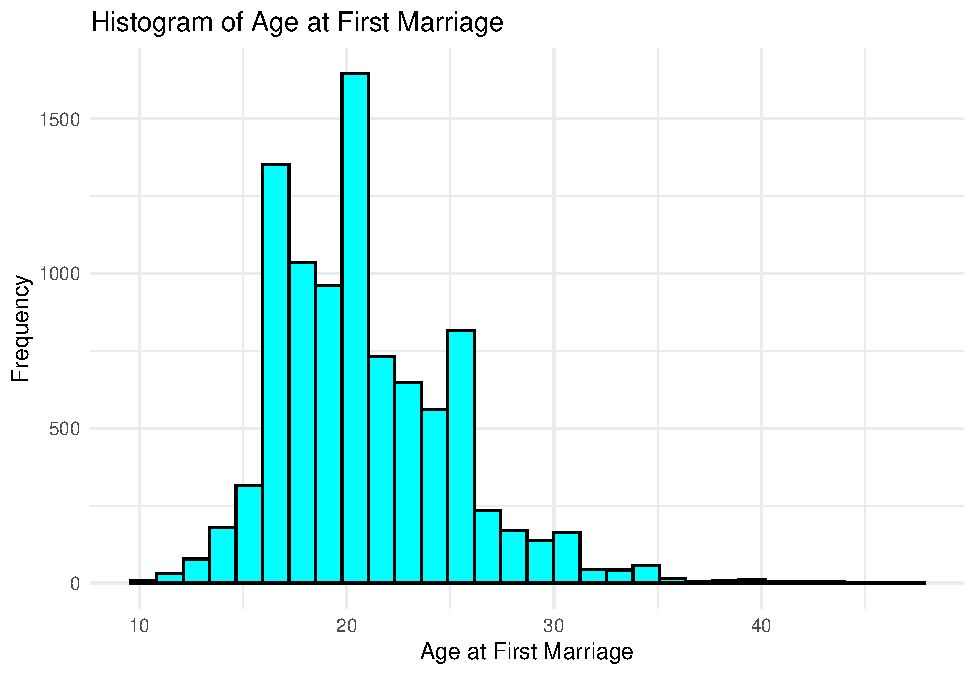
\includegraphics{ChildMarriage_files/figure-latex/unnamed-chunk-12-1.pdf}

\begin{Shaded}
\begin{Highlighting}[]
\CommentTok{\# Saving the histogram}
\CommentTok{\#ggsave("histogram\_age\_first\_marriage.png", plot = afm\_hist, width = 8, height = 6, dpi = 300)}
\end{Highlighting}
\end{Shaded}

\begin{Shaded}
\begin{Highlighting}[]
\CommentTok{\# \# Plotting a boxplot for \textquotesingle{}Age at First Marriage\textquotesingle{}}
\CommentTok{\# ggplot(female\_df, aes(y = age\_first\_marriage)) +}
\CommentTok{\#   geom\_boxplot(fill = "cyan") +}
\CommentTok{\#   labs(title = "Boxplot of Age at First Marriage", y = "Age at First Marriage") +}
\CommentTok{\#   theme\_minimal()}
\end{Highlighting}
\end{Shaded}

\begin{Shaded}
\begin{Highlighting}[]
\CommentTok{\# \# Bar plot for \textquotesingle{}used\_internet\textquotesingle{}}
\CommentTok{\# ggplot(female\_df, aes(x = used\_internet)) +}
\CommentTok{\#   geom\_bar(fill = "yellow") +}
\CommentTok{\#   theme\_minimal() +}
\CommentTok{\#   ggtitle("Bar Plot of Used Internet") +}
\CommentTok{\#   xlab("Used Internet") +}
\CommentTok{\#   ylab("Count")}
\end{Highlighting}
\end{Shaded}

\hypertarget{handling-missing-data}{%
\subsubsection{Handling Missing Data}\label{handling-missing-data}}

\begin{Shaded}
\begin{Highlighting}[]
\CommentTok{\# Before that, let\textquotesingle{}s double check the count of missing values by column}
\NormalTok{count\_missing }\OtherTok{\textless{}{-}} \FunctionTok{sapply}\NormalTok{(female\_df, }\ControlFlowTok{function}\NormalTok{(x) }\FunctionTok{sum}\NormalTok{(}\FunctionTok{is.na}\NormalTok{(x)))}
\FunctionTok{print}\NormalTok{(count\_missing)}
\end{Highlighting}
\end{Shaded}

\begin{verbatim}
##        age_first_marriage            marital_status                      area 
##                      2026                        18                        11 
##                    region           education_level          health_insurance 
##                        11                       525                       525 
##                 ethnicity              wealth_index current_contraceptive_use 
##                      1148                       524                       885 
##        awareness_hiv_aids      used_computer_tablet             used_internet 
##                       541                       532                      2501 
##         owns_mobile_phone           access_to_media 
##                       529                       529
\end{verbatim}

\begin{Shaded}
\begin{Highlighting}[]
\CommentTok{\# Make a copy of female\_df for imputation}
\NormalTok{imputed\_df }\OtherTok{\textless{}{-}}\NormalTok{ female\_df}
\end{Highlighting}
\end{Shaded}

\begin{Shaded}
\begin{Highlighting}[]
\CommentTok{\# Handle missing values in \textquotesingle{}Age at First Marriage\textquotesingle{}}

\CommentTok{\# Calculate the median value for \textquotesingle{}Age at First Marriage\textquotesingle{}, excluding NA values}
\NormalTok{median\_age\_first\_marriage }\OtherTok{\textless{}{-}} \FunctionTok{median}\NormalTok{(imputed\_df}\SpecialCharTok{$}\NormalTok{age\_first\_marriage, }\AttributeTok{na.rm =} \ConstantTok{TRUE}\NormalTok{)}

\CommentTok{\# Impute missing values in \textquotesingle{}Age at First Marriage\textquotesingle{} with the median value}
\NormalTok{imputed\_df}\SpecialCharTok{$}\NormalTok{age\_first\_marriage[}\FunctionTok{is.na}\NormalTok{(imputed\_df}\SpecialCharTok{$}\NormalTok{age\_first\_marriage)] }\OtherTok{\textless{}{-}}\NormalTok{ median\_age\_first\_marriage}
\end{Highlighting}
\end{Shaded}

\begin{Shaded}
\begin{Highlighting}[]
\CommentTok{\# Define a function to calculate mode for categorical variables}
\NormalTok{getMode }\OtherTok{\textless{}{-}} \ControlFlowTok{function}\NormalTok{(v) \{}
  \CommentTok{\# The mode is the value that appears most frequently in the data}
\NormalTok{  uniqv }\OtherTok{\textless{}{-}} \FunctionTok{unique}\NormalTok{(}\FunctionTok{na.omit}\NormalTok{(v))  }\CommentTok{\# Omit NA values and get unique values}
\NormalTok{  uniqv[}\FunctionTok{which.max}\NormalTok{(}\FunctionTok{tabulate}\NormalTok{(}\FunctionTok{match}\NormalTok{(v, uniqv)))]  }\CommentTok{\# Return the value with the highest frequency}
\NormalTok{\}}
\end{Highlighting}
\end{Shaded}

\begin{Shaded}
\begin{Highlighting}[]
\CommentTok{\# For \textquotesingle{}ethnicity\textquotesingle{}, an ordinal variable with predefined categories, it makes sense to impute missing values with the mode.}
\NormalTok{mode\_ethnicity }\OtherTok{\textless{}{-}} \FunctionTok{getMode}\NormalTok{(imputed\_df}\SpecialCharTok{$}\NormalTok{ethnicity)}
\NormalTok{imputed\_df }\OtherTok{\textless{}{-}} \FunctionTok{mutate}\NormalTok{(imputed\_df, }\AttributeTok{ethnicity =} \FunctionTok{ifelse}\NormalTok{(}\FunctionTok{is.na}\NormalTok{(ethnicity), mode\_ethnicity, ethnicity))}
\NormalTok{mode\_area }\OtherTok{\textless{}{-}} \FunctionTok{getMode}\NormalTok{(imputed\_df}\SpecialCharTok{$}\NormalTok{area)}
\NormalTok{imputed\_df }\OtherTok{\textless{}{-}} \FunctionTok{mutate}\NormalTok{(imputed\_df, }\AttributeTok{area =} \FunctionTok{ifelse}\NormalTok{(}\FunctionTok{is.na}\NormalTok{(area), mode\_area, area))}
\NormalTok{mode\_region }\OtherTok{\textless{}{-}} \FunctionTok{getMode}\NormalTok{(imputed\_df}\SpecialCharTok{$}\NormalTok{region)}
\NormalTok{imputed\_df }\OtherTok{\textless{}{-}} \FunctionTok{mutate}\NormalTok{(imputed\_df, }\AttributeTok{region =} \FunctionTok{ifelse}\NormalTok{(}\FunctionTok{is.na}\NormalTok{(region), mode\_region, region))}
\NormalTok{mode\_marital\_status }\OtherTok{\textless{}{-}} \FunctionTok{getMode}\NormalTok{(imputed\_df}\SpecialCharTok{$}\NormalTok{marital\_status)}
\NormalTok{imputed\_df }\OtherTok{\textless{}{-}} \FunctionTok{mutate}\NormalTok{(imputed\_df, }\AttributeTok{marital\_status =} \FunctionTok{ifelse}\NormalTok{(}\FunctionTok{is.na}\NormalTok{(marital\_status), mode\_marital\_status, marital\_status))}


\CommentTok{\# Binary variables like \textquotesingle{}current\_contraceptive\_use\textquotesingle{}, \textquotesingle{}health\_insurance\textquotesingle{},\textquotesingle{}awareness\_hiv\_aids\textquotesingle{}, \textquotesingle{}used\_internet\textquotesingle{}, \textquotesingle{}used\_computer\_tablet\textquotesingle{}, \textquotesingle{}owns\_mobile\_phone\textquotesingle{}, and \textquotesingle{}access\_to\_media\textquotesingle{}}
\CommentTok{\# should be imputed with the mode since it represents the most frequent category (either 0 or 1).}

\CommentTok{\# Calculate the mode for each binary variable}
\NormalTok{mode\_used\_internet }\OtherTok{\textless{}{-}} \FunctionTok{getMode}\NormalTok{(imputed\_df}\SpecialCharTok{$}\NormalTok{used\_internet)}
\NormalTok{mode\_current\_contraceptive\_use }\OtherTok{\textless{}{-}} \FunctionTok{getMode}\NormalTok{(imputed\_df}\SpecialCharTok{$}\NormalTok{current\_contraceptive\_use)}
\NormalTok{mode\_health\_insurance }\OtherTok{\textless{}{-}} \FunctionTok{getMode}\NormalTok{(imputed\_df}\SpecialCharTok{$}\NormalTok{health\_insurance)}
\NormalTok{mode\_awareness\_hiv\_aids }\OtherTok{\textless{}{-}} \FunctionTok{getMode}\NormalTok{(imputed\_df}\SpecialCharTok{$}\NormalTok{awareness\_hiv\_aids)}
\NormalTok{mode\_used\_computer\_tablet }\OtherTok{\textless{}{-}} \FunctionTok{getMode}\NormalTok{(imputed\_df}\SpecialCharTok{$}\NormalTok{used\_computer\_tablet)}
\NormalTok{mode\_owns\_mobile\_phone }\OtherTok{\textless{}{-}} \FunctionTok{getMode}\NormalTok{(imputed\_df}\SpecialCharTok{$}\NormalTok{owns\_mobile\_phone)}
\NormalTok{mode\_access\_to\_media }\OtherTok{\textless{}{-}} \FunctionTok{getMode}\NormalTok{(imputed\_df}\SpecialCharTok{$}\NormalTok{access\_to\_media)}

\CommentTok{\# Impute missing values for binary variables}
\NormalTok{imputed\_df }\OtherTok{\textless{}{-}} \FunctionTok{mutate}\NormalTok{(imputed\_df,}
  \AttributeTok{used\_internet =} \FunctionTok{ifelse}\NormalTok{(}\FunctionTok{is.na}\NormalTok{(used\_internet), mode\_used\_internet, used\_internet),}
  \AttributeTok{current\_contraceptive\_use =} \FunctionTok{ifelse}\NormalTok{(}\FunctionTok{is.na}\NormalTok{(current\_contraceptive\_use), mode\_current\_contraceptive\_use, current\_contraceptive\_use),}
  \AttributeTok{health\_insurance =} \FunctionTok{ifelse}\NormalTok{(}\FunctionTok{is.na}\NormalTok{(health\_insurance), mode\_health\_insurance, health\_insurance),}
  \AttributeTok{awareness\_hiv\_aids =} \FunctionTok{ifelse}\NormalTok{(}\FunctionTok{is.na}\NormalTok{(awareness\_hiv\_aids), mode\_awareness\_hiv\_aids, awareness\_hiv\_aids),}
  \AttributeTok{used\_computer\_tablet =} \FunctionTok{ifelse}\NormalTok{(}\FunctionTok{is.na}\NormalTok{(used\_computer\_tablet), mode\_used\_computer\_tablet, used\_computer\_tablet),}
  \AttributeTok{owns\_mobile\_phone =} \FunctionTok{ifelse}\NormalTok{(}\FunctionTok{is.na}\NormalTok{(owns\_mobile\_phone), mode\_owns\_mobile\_phone, owns\_mobile\_phone),}
  \AttributeTok{access\_to\_media =} \FunctionTok{ifelse}\NormalTok{(}\FunctionTok{is.na}\NormalTok{(access\_to\_media), mode\_access\_to\_media, access\_to\_media)}
\NormalTok{)}

\CommentTok{\# \textquotesingle{}education\_level\textquotesingle{} is an ordinal variable where the median could be a more suitable measure of central tendency than the mode.}
\CommentTok{\# However, given the categorical nature of the levels (e.g., "Primary", "Secondary"), using the mode may still be appropriate.}
\NormalTok{mode\_education\_level }\OtherTok{\textless{}{-}} \FunctionTok{getMode}\NormalTok{(imputed\_df}\SpecialCharTok{$}\NormalTok{education\_level)}
\NormalTok{imputed\_df }\OtherTok{\textless{}{-}} \FunctionTok{mutate}\NormalTok{(imputed\_df, }\AttributeTok{education\_level =} \FunctionTok{ifelse}\NormalTok{(}\FunctionTok{is.na}\NormalTok{(education\_level), mode\_education\_level, education\_level))}

\CommentTok{\# \textquotesingle{}wealth\_index\textquotesingle{} is an ordinal variable where the median could be a more suitable measure of central tendency than the mode.}
\CommentTok{\# However, given the categorical nature of the levels (e.g., "Poorest", "Poor",...), using the mode may still be appropriate.}
\NormalTok{mode\_wealth\_index }\OtherTok{\textless{}{-}} \FunctionTok{getMode}\NormalTok{(imputed\_df}\SpecialCharTok{$}\NormalTok{wealth\_index)}
\NormalTok{imputed\_df }\OtherTok{\textless{}{-}} \FunctionTok{mutate}\NormalTok{(imputed\_df, }\AttributeTok{wealth\_index =} \FunctionTok{ifelse}\NormalTok{(}\FunctionTok{is.na}\NormalTok{(wealth\_index), mode\_wealth\_index, wealth\_index))}
\end{Highlighting}
\end{Shaded}

\begin{Shaded}
\begin{Highlighting}[]
\CommentTok{\# Check the resulting dataset to confirm changes}
\FunctionTok{summary}\NormalTok{(imputed\_df)}
\end{Highlighting}
\end{Shaded}

\begin{verbatim}
##  age_first_marriage marital_status       area           region     
##  Min.   :10.00      Min.   :1.000   Min.   :1.000   Min.   :1.000  
##  1st Qu.:18.00      1st Qu.:1.000   1st Qu.:1.000   1st Qu.:2.000  
##  Median :20.00      Median :1.000   Median :2.000   Median :3.000  
##  Mean   :20.76      Mean   :1.408   Mean   :1.684   Mean   :3.403  
##  3rd Qu.:23.00      3rd Qu.:1.000   3rd Qu.:2.000   3rd Qu.:5.000  
##  Max.   :47.00      Max.   :3.000   Max.   :2.000   Max.   :6.000  
##  education_level health_insurance   ethnicity      wealth_index 
##  Min.   :0.000   Min.   :0.0000   Min.   :1.000   Min.   :1.00  
##  1st Qu.:1.000   1st Qu.:1.0000   1st Qu.:1.000   1st Qu.:1.00  
##  Median :2.000   Median :1.0000   Median :1.000   Median :2.00  
##  Mean   :2.438   Mean   :0.8721   Mean   :1.527   Mean   :2.54  
##  3rd Qu.:3.000   3rd Qu.:1.0000   3rd Qu.:2.000   3rd Qu.:4.00  
##  Max.   :5.000   Max.   :1.0000   Max.   :4.000   Max.   :5.00  
##  current_contraceptive_use awareness_hiv_aids used_computer_tablet
##  Min.   :0.0000            Min.   :0.0000     Min.   :0.0000      
##  1st Qu.:0.0000            1st Qu.:1.0000     1st Qu.:0.0000      
##  Median :1.0000            Median :1.0000     Median :0.0000      
##  Mean   :0.6168            Mean   :0.8072     Mean   :0.3251      
##  3rd Qu.:1.0000            3rd Qu.:1.0000     3rd Qu.:1.0000      
##  Max.   :1.0000            Max.   :1.0000     Max.   :1.0000      
##  used_internet    owns_mobile_phone access_to_media 
##  Min.   :0.0000   Min.   :0.0000    Min.   :0.0000  
##  1st Qu.:0.0000   1st Qu.:1.0000    1st Qu.:1.0000  
##  Median :1.0000   Median :1.0000    Median :1.0000  
##  Mean   :0.7192   Mean   :0.8886    Mean   :0.9071  
##  3rd Qu.:1.0000   3rd Qu.:1.0000    3rd Qu.:1.0000  
##  Max.   :1.0000   Max.   :1.0000    Max.   :1.0000
\end{verbatim}

\begin{Shaded}
\begin{Highlighting}[]
\CommentTok{\# After imputation, let\textquotesingle{}s check for missing values}
\NormalTok{count\_imputation }\OtherTok{\textless{}{-}} \FunctionTok{sapply}\NormalTok{(imputed\_df, }\ControlFlowTok{function}\NormalTok{(x) }\FunctionTok{sum}\NormalTok{(}\FunctionTok{is.na}\NormalTok{(x)))}
\FunctionTok{print}\NormalTok{(count\_imputation)}
\end{Highlighting}
\end{Shaded}

\begin{verbatim}
##        age_first_marriage            marital_status                      area 
##                         0                         0                         0 
##                    region           education_level          health_insurance 
##                         0                         0                         0 
##                 ethnicity              wealth_index current_contraceptive_use 
##                         0                         0                         0 
##        awareness_hiv_aids      used_computer_tablet             used_internet 
##                         0                         0                         0 
##         owns_mobile_phone           access_to_media 
##                         0                         0
\end{verbatim}

\hypertarget{visualization-comparing-before-vs.-after-imputation}{%
\subsubsection{Visualization Comparing Before vs.~After
Imputation}\label{visualization-comparing-before-vs.-after-imputation}}

\begin{Shaded}
\begin{Highlighting}[]
\CommentTok{\# Histogram for \textquotesingle{}age\_first\_marriage\textquotesingle{} before imputation}
\NormalTok{afm\_0 }\OtherTok{\textless{}{-}} \FunctionTok{ggplot}\NormalTok{(female\_df, }\FunctionTok{aes}\NormalTok{(}\AttributeTok{x =}\NormalTok{ age\_first\_marriage)) }\SpecialCharTok{+} 
  \FunctionTok{geom\_histogram}\NormalTok{(}\AttributeTok{fill =} \StringTok{"lightpink"}\NormalTok{, }\AttributeTok{color =} \StringTok{"black"}\NormalTok{, }\AttributeTok{bins =} \DecValTok{30}\NormalTok{) }\SpecialCharTok{+}
  \FunctionTok{theme\_light}\NormalTok{() }\SpecialCharTok{+}
  \FunctionTok{ggtitle}\NormalTok{(}\StringTok{"Age at First Marriage Before Imputation"}\NormalTok{) }\SpecialCharTok{+}
  \FunctionTok{xlab}\NormalTok{(}\StringTok{"Age at First Marriage"}\NormalTok{) }\SpecialCharTok{+}
  \FunctionTok{ylab}\NormalTok{(}\StringTok{"Frequency"}\NormalTok{)}

\CommentTok{\# Histogram for \textquotesingle{}age\_first\_marriage\textquotesingle{} after imputation}
\NormalTok{afm\_imputed }\OtherTok{\textless{}{-}} \FunctionTok{ggplot}\NormalTok{(imputed\_df, }\FunctionTok{aes}\NormalTok{(}\AttributeTok{x =}\NormalTok{ age\_first\_marriage)) }\SpecialCharTok{+} 
  \FunctionTok{geom\_histogram}\NormalTok{(}\AttributeTok{fill =} \StringTok{"plum"}\NormalTok{, }\AttributeTok{color =} \StringTok{"black"}\NormalTok{, }\AttributeTok{bins =} \DecValTok{30}\NormalTok{) }\SpecialCharTok{+}
  \FunctionTok{theme\_light}\NormalTok{() }\SpecialCharTok{+}
  \FunctionTok{ggtitle}\NormalTok{(}\StringTok{"Age at First Marriage After Imputation"}\NormalTok{) }\SpecialCharTok{+}
  \FunctionTok{xlab}\NormalTok{(}\StringTok{"Age at First Marriage"}\NormalTok{) }\SpecialCharTok{+}
  \FunctionTok{ylab}\NormalTok{(}\StringTok{"Frequency"}\NormalTok{)}

\CommentTok{\# Arrange the two plots side by side}
\FunctionTok{grid.arrange}\NormalTok{(afm\_0, afm\_imputed, }\AttributeTok{ncol =} \DecValTok{2}\NormalTok{)}
\end{Highlighting}
\end{Shaded}

\begin{verbatim}
## Warning: Removed 2026 rows containing non-finite outside the scale range
## (`stat_bin()`).
\end{verbatim}

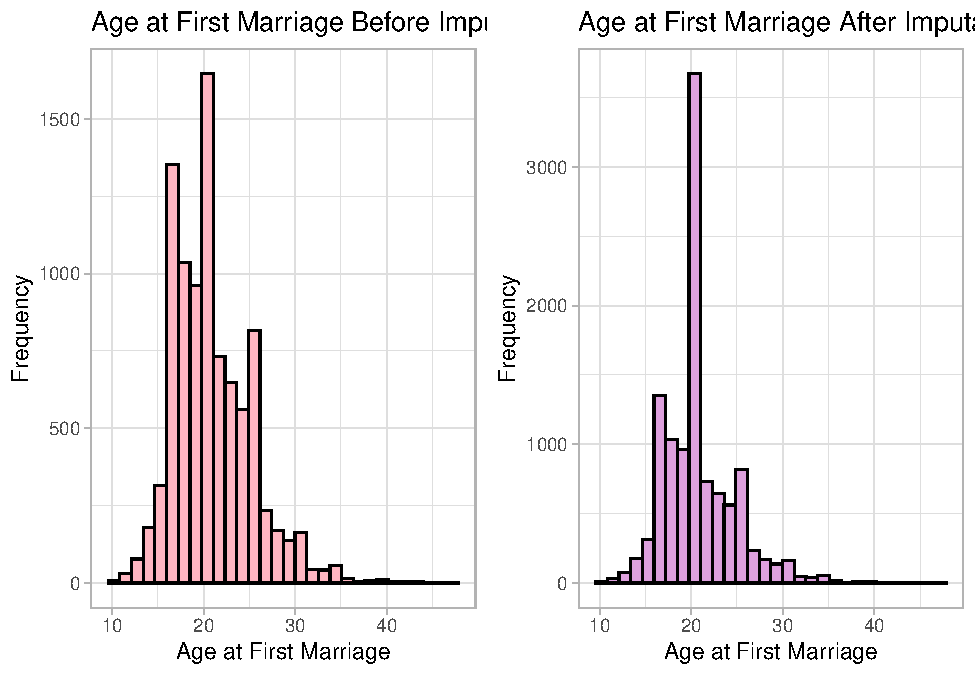
\includegraphics{ChildMarriage_files/figure-latex/unnamed-chunk-23-1.pdf}

\begin{Shaded}
\begin{Highlighting}[]
\CommentTok{\# Arrange the two plots side by side and capture the layout as a grob}
\NormalTok{combined\_plots }\OtherTok{\textless{}{-}} \FunctionTok{arrangeGrob}\NormalTok{(afm\_0, afm\_imputed, }\AttributeTok{ncol =} \DecValTok{2}\NormalTok{)}
\end{Highlighting}
\end{Shaded}

\begin{verbatim}
## Warning: Removed 2026 rows containing non-finite outside the scale range
## (`stat_bin()`).
\end{verbatim}

\begin{Shaded}
\begin{Highlighting}[]
\CommentTok{\# Now, use ggsave to save the combined plot}
\CommentTok{\#ggsave("combined\_age\_first\_marriage.png", plot = combined\_plots, width = 10, height = 5)}
\end{Highlighting}
\end{Shaded}

\hypertarget{creating-binary-variables-for-child-marriage-under-18-and-16}{%
\subsubsection{Creating Binary Variables for Child Marriage Under 18 and
16}\label{creating-binary-variables-for-child-marriage-under-18-and-16}}

\begin{Shaded}
\begin{Highlighting}[]
\CommentTok{\# Convert "age at first marriage" into a binary variable to indicate child marriage}
\CommentTok{\# Child marriage is defined as marriage before the age of 18}
\CommentTok{\# The new binary variable "child\_marriage" will have a value of 1 if the marriage occurred before age 18, and 0 otherwise}
\NormalTok{imputed\_df }\OtherTok{\textless{}{-}}\NormalTok{ imputed\_df }\SpecialCharTok{\%\textgreater{}\%}
  \FunctionTok{mutate}\NormalTok{(}\AttributeTok{child\_marriage =} \FunctionTok{ifelse}\NormalTok{(age\_first\_marriage }\SpecialCharTok{\textless{}} \DecValTok{18}\NormalTok{, }\DecValTok{1}\NormalTok{, }\DecValTok{0}\NormalTok{))}
\end{Highlighting}
\end{Shaded}

\begin{Shaded}
\begin{Highlighting}[]
\CommentTok{\# Create a binary variable for child marriage under 16}
\CommentTok{\# The new variable "child\_marriage\_u16" will have a value of 1 if the marriage occurred before age 16, and 0 otherwise}
\NormalTok{imputed\_df }\OtherTok{\textless{}{-}}\NormalTok{ imputed\_df }\SpecialCharTok{\%\textgreater{}\%}
  \FunctionTok{mutate}\NormalTok{(}\AttributeTok{child\_marriage\_u16 =} \FunctionTok{ifelse}\NormalTok{(age\_first\_marriage }\SpecialCharTok{\textless{}} \DecValTok{16}\NormalTok{, }\DecValTok{1}\NormalTok{, }\DecValTok{0}\NormalTok{))}
\end{Highlighting}
\end{Shaded}

\begin{Shaded}
\begin{Highlighting}[]
\CommentTok{\# Move "child\_marriage" and "child\_marriage\_u16" to the front of the dataframe}
\NormalTok{imputed\_df }\OtherTok{\textless{}{-}}\NormalTok{ imputed\_df }\SpecialCharTok{\%\textgreater{}\%}
  \FunctionTok{select}\NormalTok{(child\_marriage, child\_marriage\_u16, }\FunctionTok{everything}\NormalTok{())}
\end{Highlighting}
\end{Shaded}

\begin{Shaded}
\begin{Highlighting}[]
\CommentTok{\# Exporting female\_df to a CSV file in the current working directory}
\FunctionTok{write.csv}\NormalTok{(imputed\_df, }\StringTok{"imputed\_df.csv"}\NormalTok{, }\AttributeTok{row.names =} \ConstantTok{FALSE}\NormalTok{)}
\end{Highlighting}
\end{Shaded}

\hypertarget{eda}{%
\subsubsection{EDA}\label{eda}}

\begin{Shaded}
\begin{Highlighting}[]
\CommentTok{\# Calculate total observations}
\NormalTok{total\_obs }\OtherTok{\textless{}{-}} \FunctionTok{nrow}\NormalTok{(imputed\_df)}

\CommentTok{\# Aggregate counts for each category by region without altering the original \textquotesingle{}region\textquotesingle{} field}
\NormalTok{counts\_df }\OtherTok{\textless{}{-}} \FunctionTok{aggregate}\NormalTok{(}\FunctionTok{cbind}\NormalTok{(}\AttributeTok{ever\_married =}\NormalTok{ imputed\_df}\SpecialCharTok{$}\NormalTok{marital\_status }\SpecialCharTok{\%in\%} \FunctionTok{c}\NormalTok{(}\DecValTok{1}\NormalTok{, }\DecValTok{2}\NormalTok{), }
                             \AttributeTok{married\_u18 =}\NormalTok{ imputed\_df}\SpecialCharTok{$}\NormalTok{child\_marriage }\SpecialCharTok{==} \DecValTok{1}\NormalTok{, }
                             \AttributeTok{married\_u16 =}\NormalTok{ imputed\_df}\SpecialCharTok{$}\NormalTok{child\_marriage\_u16 }\SpecialCharTok{==} \DecValTok{1}\NormalTok{) }\SpecialCharTok{\textasciitilde{}}\NormalTok{ region, }
                       \AttributeTok{data =}\NormalTok{ imputed\_df, }
                       \AttributeTok{FUN =}\NormalTok{ sum)}

\CommentTok{\# Convert counts to percentages}
\NormalTok{counts\_df}\SpecialCharTok{$}\NormalTok{ever\_married }\OtherTok{\textless{}{-}}\NormalTok{ (counts\_df}\SpecialCharTok{$}\NormalTok{ever\_married }\SpecialCharTok{/}\NormalTok{ total\_obs) }\SpecialCharTok{*} \DecValTok{100}
\NormalTok{counts\_df}\SpecialCharTok{$}\NormalTok{married\_u18 }\OtherTok{\textless{}{-}}\NormalTok{ (counts\_df}\SpecialCharTok{$}\NormalTok{married\_u18 }\SpecialCharTok{/}\NormalTok{ total\_obs) }\SpecialCharTok{*} \DecValTok{100}
\NormalTok{counts\_df}\SpecialCharTok{$}\NormalTok{married\_u16 }\OtherTok{\textless{}{-}}\NormalTok{ (counts\_df}\SpecialCharTok{$}\NormalTok{married\_u16 }\SpecialCharTok{/}\NormalTok{ total\_obs) }\SpecialCharTok{*} \DecValTok{100}


\CommentTok{\# Creating the plot with ggplot2, directly labeling regions}
\NormalTok{p }\OtherTok{\textless{}{-}} \FunctionTok{ggplot}\NormalTok{(counts\_df, }\FunctionTok{aes}\NormalTok{(}\AttributeTok{x =} \FunctionTok{factor}\NormalTok{(region))) }\SpecialCharTok{+}
  \FunctionTok{geom\_bar}\NormalTok{(}\FunctionTok{aes}\NormalTok{(}\AttributeTok{y =}\NormalTok{ ever\_married, }\AttributeTok{fill =} \StringTok{"Ever married or cohabited"}\NormalTok{), }\AttributeTok{stat =} \StringTok{"identity"}\NormalTok{) }\SpecialCharTok{+}
  \FunctionTok{geom\_bar}\NormalTok{(}\FunctionTok{aes}\NormalTok{(}\AttributeTok{y =}\NormalTok{ married\_u18, }\AttributeTok{fill =} \StringTok{"Married or cohabited before 18 years old"}\NormalTok{), }\AttributeTok{stat =} \StringTok{"identity"}\NormalTok{) }\SpecialCharTok{+}
  \FunctionTok{geom\_bar}\NormalTok{(}\FunctionTok{aes}\NormalTok{(}\AttributeTok{y =}\NormalTok{ married\_u16, }\AttributeTok{fill =} \StringTok{"Married or cohabited before 16 years old"}\NormalTok{), }\AttributeTok{stat =} \StringTok{"identity"}\NormalTok{) }\SpecialCharTok{+}
  \FunctionTok{scale\_fill\_manual}\NormalTok{(}\AttributeTok{values =} \FunctionTok{c}\NormalTok{(}\StringTok{"Ever married or cohabited"} \OtherTok{=} \StringTok{"snow2"}\NormalTok{, }
                               \StringTok{"Married or cohabited before 18 years old"} \OtherTok{=} \StringTok{"grey"}\NormalTok{, }
                               \StringTok{"Married or cohabited before 16 years old"} \OtherTok{=} \StringTok{"black"}\NormalTok{),}
                    \AttributeTok{name =} \StringTok{"Marital Status"}\NormalTok{) }\SpecialCharTok{+}
  \FunctionTok{labs}\NormalTok{(}\AttributeTok{x =} \StringTok{"Region"}\NormalTok{, }\AttributeTok{y =} \StringTok{"Percentage"}\NormalTok{, }\AttributeTok{title =} \StringTok{"Prevalence of Child Marriage by Regions Among Females"}\NormalTok{) }\SpecialCharTok{+}
  \FunctionTok{theme\_minimal}\NormalTok{() }\SpecialCharTok{+}
  \FunctionTok{theme}\NormalTok{(}\AttributeTok{plot.margin =} \FunctionTok{margin}\NormalTok{(}\AttributeTok{t =} \DecValTok{10}\NormalTok{, }\AttributeTok{r =} \DecValTok{10}\NormalTok{, }\AttributeTok{b =} \DecValTok{10}\NormalTok{, }\AttributeTok{l =} \DecValTok{10}\NormalTok{, }\AttributeTok{unit =} \StringTok{"mm"}\NormalTok{), }
        \AttributeTok{axis.text.x =} \FunctionTok{element\_text}\NormalTok{(}\AttributeTok{angle =} \DecValTok{45}\NormalTok{, }\AttributeTok{hjust =} \DecValTok{1}\NormalTok{), }
        \AttributeTok{legend.position =} \StringTok{"right"}\NormalTok{) }\SpecialCharTok{+}
  \FunctionTok{scale\_x\_discrete}\NormalTok{(}\AttributeTok{labels =} \FunctionTok{c}\NormalTok{(}\StringTok{"1"} \OtherTok{=} \StringTok{"Red River Delta"}\NormalTok{, }\StringTok{"2"} \OtherTok{=} \StringTok{"Northern Midlands And Mountain"}\NormalTok{, }
                              \StringTok{"3"} \OtherTok{=} \StringTok{"North Central And Central Coastal"}\NormalTok{, }\StringTok{"4"} \OtherTok{=} \StringTok{"Central Highlands"}\NormalTok{, }
                              \StringTok{"5"} \OtherTok{=} \StringTok{"South East"}\NormalTok{, }\StringTok{"6"} \OtherTok{=} \StringTok{"Mekong River Delta"}\NormalTok{))}

\CommentTok{\# Convert ggplot object to plotly for interactive visualization}
\FunctionTok{ggplotly}\NormalTok{(p)}
\end{Highlighting}
\end{Shaded}

\includegraphics{ChildMarriage_files/figure-latex/unnamed-chunk-29-1.pdf}

\hypertarget{preparing-for-regression-analysis}{%
\subsubsection{Preparing for Regression
Analysis}\label{preparing-for-regression-analysis}}

\hypertarget{correlation-matrix}{%
\paragraph{Correlation Matrix}\label{correlation-matrix}}

\begin{Shaded}
\begin{Highlighting}[]
\CommentTok{\# Calculate correlation matrix}
\NormalTok{cor\_matrix }\OtherTok{\textless{}{-}} \FunctionTok{cor}\NormalTok{(imputed\_df }\SpecialCharTok{\%\textgreater{}\%} \FunctionTok{select\_if}\NormalTok{(is.numeric), }\AttributeTok{use =} \StringTok{"complete.obs"}\NormalTok{)}

\CommentTok{\# Melt the correlation matrix}
\NormalTok{melted\_cor\_matrix }\OtherTok{\textless{}{-}} \FunctionTok{melt}\NormalTok{(cor\_matrix)}
\end{Highlighting}
\end{Shaded}

\begin{Shaded}
\begin{Highlighting}[]
\CommentTok{\# Generate an interactive heatmap}
\NormalTok{corr\_matrix }\OtherTok{\textless{}{-}} \FunctionTok{ggplot}\NormalTok{(melted\_cor\_matrix, }\FunctionTok{aes}\NormalTok{(Var1, Var2, }\AttributeTok{fill =}\NormalTok{ value)) }\SpecialCharTok{+}
    \FunctionTok{geom\_tile}\NormalTok{() }\SpecialCharTok{+}
    \FunctionTok{scale\_fill\_gradientn}\NormalTok{(}
        \AttributeTok{colours =} \FunctionTok{c}\NormalTok{(}\StringTok{"deepskyblue"}\NormalTok{, }\StringTok{"white"}\NormalTok{, }\StringTok{"red2"}\NormalTok{),}
        \AttributeTok{values =}\NormalTok{ scales}\SpecialCharTok{::}\FunctionTok{rescale}\NormalTok{(}\FunctionTok{c}\NormalTok{(}\SpecialCharTok{{-}}\DecValTok{1}\NormalTok{, }\DecValTok{0}\NormalTok{, }\DecValTok{1}\NormalTok{)),}
        \AttributeTok{limits =} \FunctionTok{c}\NormalTok{(}\SpecialCharTok{{-}}\DecValTok{1}\NormalTok{, }\DecValTok{1}\NormalTok{),}
        \AttributeTok{name=}\StringTok{"Pearson}\SpecialCharTok{\textbackslash{}n}\StringTok{Correlation"}
\NormalTok{    ) }\SpecialCharTok{+}
    \FunctionTok{theme\_minimal}\NormalTok{() }\SpecialCharTok{+} 
    \FunctionTok{theme}\NormalTok{(}\AttributeTok{axis.text.x =} \FunctionTok{element\_text}\NormalTok{(}\AttributeTok{angle =} \DecValTok{45}\NormalTok{, }\AttributeTok{hjust =} \DecValTok{1}\NormalTok{)) }\SpecialCharTok{+}
    \FunctionTok{xlab}\NormalTok{(}\StringTok{""}\NormalTok{) }\SpecialCharTok{+} 
    \FunctionTok{ylab}\NormalTok{(}\StringTok{""}\NormalTok{) }\SpecialCharTok{+}
    \FunctionTok{ggtitle}\NormalTok{(}\StringTok{"Correlation Matrix"}\NormalTok{) }

\CommentTok{\# Convert ggplot object to plotly for interactivity}
\FunctionTok{ggplotly}\NormalTok{(corr\_matrix)}
\end{Highlighting}
\end{Shaded}

\includegraphics{ChildMarriage_files/figure-latex/unnamed-chunk-32-1.pdf}

\hypertarget{converting-categorical-and-binary-variables-to-factors}{%
\paragraph{Converting Categorical and Binary Variables to
Factors}\label{converting-categorical-and-binary-variables-to-factors}}

\begin{Shaded}
\begin{Highlighting}[]
\CommentTok{\# \# Mapping for \textquotesingle{}area\textquotesingle{}}
\CommentTok{\# area\_labels \textless{}{-} c("Urban", "Rural")}
\CommentTok{\# names(area\_labels) \textless{}{-} c("1", "2")}
\CommentTok{\# }
\CommentTok{\# \# Mapping for \textquotesingle{}region\textquotesingle{}}
\CommentTok{\# region\_labels \textless{}{-} c("Red River Delta", "Northern Midlands And Mountain", "North Central And Central Coastal", "Central Highlands", "South East", "Mekong River Delta")}
\CommentTok{\# names(region\_labels) \textless{}{-} c("1", "2", "3", "4", "5", "6")}
\CommentTok{\# }
\CommentTok{\# \# Mapping for \textquotesingle{}education\_level\textquotesingle{}}
\CommentTok{\# education\_level\_labels \textless{}{-} c("None or Pre{-}Primary", "Primary", "Lower Primary", "Upper Primary", "Vocational High School", "University/College/Higher")}
\CommentTok{\# names(education\_level\_labels) \textless{}{-} c("0", "1", "2", "3", "4", "5") }
\CommentTok{\# }
\CommentTok{\# \# Mapping for \textquotesingle{}ethnicity\textquotesingle{}}
\CommentTok{\# ethnicity\_labels \textless{}{-} c("Kinh and Hoa", "Tay, Thai, Muong, Nung", "Khmer", "Mong")  \# Add or modify as per your dataset}
\CommentTok{\# names(ethnicity\_labels) \textless{}{-} c("1", "2", "3", "4")  }
\CommentTok{\# }
\CommentTok{\# \# Mapping for \textquotesingle{}wealth\_index\textquotesingle{}}
\CommentTok{\# wealth\_index\_labels \textless{}{-} c("Poorest", "Poor", "Middle", "Rich", "Richest")}
\CommentTok{\# names(wealth\_index\_labels) \textless{}{-} c("1", "2", "3", "4", "5") }
\end{Highlighting}
\end{Shaded}

\begin{Shaded}
\begin{Highlighting}[]
\CommentTok{\# Convert nominal and ordinal variables to factors}
\NormalTok{imputed\_df}\SpecialCharTok{$}\NormalTok{area }\OtherTok{\textless{}{-}} \FunctionTok{as.factor}\NormalTok{(imputed\_df}\SpecialCharTok{$}\NormalTok{area)}
\NormalTok{imputed\_df}\SpecialCharTok{$}\NormalTok{region }\OtherTok{\textless{}{-}} \FunctionTok{as.factor}\NormalTok{(imputed\_df}\SpecialCharTok{$}\NormalTok{region)}
\NormalTok{imputed\_df}\SpecialCharTok{$}\NormalTok{education\_level }\OtherTok{\textless{}{-}} \FunctionTok{factor}\NormalTok{(imputed\_df}\SpecialCharTok{$}\NormalTok{education\_level, }\AttributeTok{ordered =} \ConstantTok{FALSE}\NormalTok{)}
\NormalTok{imputed\_df}\SpecialCharTok{$}\NormalTok{ethnicity }\OtherTok{\textless{}{-}} \FunctionTok{as.factor}\NormalTok{(imputed\_df}\SpecialCharTok{$}\NormalTok{ethnicity)}
\NormalTok{imputed\_df}\SpecialCharTok{$}\NormalTok{wealth\_index }\OtherTok{\textless{}{-}} \FunctionTok{factor}\NormalTok{(imputed\_df}\SpecialCharTok{$}\NormalTok{wealth\_index, }\AttributeTok{ordered =} \ConstantTok{FALSE}\NormalTok{)}

\CommentTok{\# Binary variables are already in the correct format and can be used as is}
\end{Highlighting}
\end{Shaded}

\hypertarget{base-logistic-regression-model}{%
\subsubsection{Base Logistic Regression
Model}\label{base-logistic-regression-model}}

\begin{Shaded}
\begin{Highlighting}[]
\CommentTok{\# Baseline model for reference}
\NormalTok{baseline\_model }\OtherTok{\textless{}{-}} \FunctionTok{glm}\NormalTok{(child\_marriage }\SpecialCharTok{\textasciitilde{}}\NormalTok{ area }\SpecialCharTok{+}\NormalTok{ education\_level }\SpecialCharTok{+}\NormalTok{ wealth\_index }\SpecialCharTok{+}\NormalTok{ health\_insurance }\SpecialCharTok{+}\NormalTok{ current\_contraceptive\_use }\SpecialCharTok{+}\NormalTok{ awareness\_hiv\_aids }\SpecialCharTok{+}\NormalTok{ access\_to\_media, }\AttributeTok{family =} \FunctionTok{binomial}\NormalTok{(), }\AttributeTok{data =}\NormalTok{ imputed\_df)}

\CommentTok{\# Summarize the baseline model}
\FunctionTok{summary}\NormalTok{(baseline\_model)}
\end{Highlighting}
\end{Shaded}

\begin{verbatim}
## 
## Call:
## glm(formula = child_marriage ~ area + education_level + wealth_index + 
##     health_insurance + current_contraceptive_use + awareness_hiv_aids + 
##     access_to_media, family = binomial(), data = imputed_df)
## 
## Coefficients:
##                           Estimate Std. Error z value Pr(>|z|)    
## (Intercept)               -0.73391    0.13169  -5.573 2.50e-08 ***
## area2                      0.45543    0.07999   5.693 1.25e-08 ***
## education_level1          -0.41350    0.08705  -4.750 2.03e-06 ***
## education_level2          -0.58693    0.08518  -6.890 5.57e-12 ***
## education_level3          -1.52807    0.11502 -13.286  < 2e-16 ***
## education_level4          -3.24812    0.51198  -6.344 2.24e-10 ***
## education_level5          -3.19482    0.25323 -12.616  < 2e-16 ***
## wealth_index2             -0.46183    0.07994  -5.777 7.61e-09 ***
## wealth_index3             -0.80552    0.09964  -8.085 6.24e-16 ***
## wealth_index4             -0.61389    0.10926  -5.618 1.93e-08 ***
## wealth_index5             -0.89341    0.14898  -5.997 2.01e-09 ***
## health_insurance           0.06907    0.08094   0.853    0.393    
## current_contraceptive_use  0.40123    0.06065   6.615 3.71e-11 ***
## awareness_hiv_aids        -0.47875    0.06960  -6.879 6.05e-12 ***
## access_to_media           -0.01461    0.08121  -0.180    0.857    
## ---
## Signif. codes:  0 '***' 0.001 '**' 0.01 '*' 0.05 '.' 0.1 ' ' 1
## 
## (Dispersion parameter for binomial family taken to be 1)
## 
##     Null deviance: 10439.1  on 11293  degrees of freedom
## Residual deviance:  8493.7  on 11279  degrees of freedom
## AIC: 8523.7
## 
## Number of Fisher Scoring iterations: 7
\end{verbatim}

\hypertarget{accessing-base-models-multicollinearity}{%
\paragraph{Accessing Base Model's
Multicollinearity}\label{accessing-base-models-multicollinearity}}

\begin{Shaded}
\begin{Highlighting}[]
\CommentTok{\# Calculate VIF (A VIF value \textgreater{} 5 indicates high multicollinearity)}
\NormalTok{base\_vif\_results }\OtherTok{\textless{}{-}} \FunctionTok{vif}\NormalTok{(baseline\_model)}
\FunctionTok{print}\NormalTok{(base\_vif\_results)}
\end{Highlighting}
\end{Shaded}

\begin{verbatim}
##                               GVIF Df GVIF^(1/(2*Df))
## area                      1.110732  1        1.053913
## education_level           1.707863  5        1.054983
## wealth_index              1.401192  4        1.043067
## health_insurance          1.021120  1        1.010505
## current_contraceptive_use 1.034853  1        1.017277
## awareness_hiv_aids        1.500511  1        1.224954
## access_to_media           1.268704  1        1.126367
\end{verbatim}

\begin{Shaded}
\begin{Highlighting}[]
\CommentTok{\# Check if any VIF value is greater than a typical threshold, like 5 or 10.}
\NormalTok{base\_high\_vif }\OtherTok{\textless{}{-}}\NormalTok{ base\_vif\_results[base\_vif\_results }\SpecialCharTok{\textgreater{}} \DecValTok{5}\NormalTok{]}
\FunctionTok{print}\NormalTok{(base\_high\_vif)}
\end{Highlighting}
\end{Shaded}

\begin{verbatim}
## numeric(0)
\end{verbatim}

\hypertarget{adding-fixed-effects-to-base-model}{%
\subsubsection{Adding Fixed Effects to Base
Model}\label{adding-fixed-effects-to-base-model}}

\begin{Shaded}
\begin{Highlighting}[]
\CommentTok{\# Enhanced model with additional fixed effects}
\NormalTok{enhanced\_model }\OtherTok{\textless{}{-}} \FunctionTok{glm}\NormalTok{(child\_marriage }\SpecialCharTok{\textasciitilde{}}\NormalTok{ area }\SpecialCharTok{+}\NormalTok{ region }\SpecialCharTok{+}\NormalTok{ education\_level }\SpecialCharTok{+}\NormalTok{ ethnicity }\SpecialCharTok{+}\NormalTok{ wealth\_index }\SpecialCharTok{+}\NormalTok{ health\_insurance }\SpecialCharTok{+}\NormalTok{ current\_contraceptive\_use }\SpecialCharTok{+}\NormalTok{ awareness\_hiv\_aids }\SpecialCharTok{+}\NormalTok{ access\_to\_media, }
                      \AttributeTok{family =} \FunctionTok{binomial}\NormalTok{(), }
                      \AttributeTok{data =}\NormalTok{ imputed\_df)}

\CommentTok{\# Summarize the new model with FEs}
\FunctionTok{summary}\NormalTok{(enhanced\_model)}
\end{Highlighting}
\end{Shaded}

\begin{verbatim}
## 
## Call:
## glm(formula = child_marriage ~ area + region + education_level + 
##     ethnicity + wealth_index + health_insurance + current_contraceptive_use + 
##     awareness_hiv_aids + access_to_media, family = binomial(), 
##     data = imputed_df)
## 
## Coefficients:
##                           Estimate Std. Error z value Pr(>|z|)    
## (Intercept)               -1.54522    0.17906  -8.630  < 2e-16 ***
## area2                      0.28689    0.08488   3.380 0.000725 ***
## region2                    0.37758    0.12919   2.923 0.003469 ** 
## region3                    0.18170    0.12745   1.426 0.153967    
## region4                    0.34057    0.12599   2.703 0.006869 ** 
## region5                   -0.05340    0.12612  -0.423 0.672028    
## region6                   -0.05277    0.13336  -0.396 0.692301    
## education_level1          -0.05925    0.09353  -0.634 0.526382    
## education_level2          -0.22571    0.09227  -2.446 0.014438 *  
## education_level3          -1.17196    0.12172  -9.629  < 2e-16 ***
## education_level4          -2.96956    0.51385  -5.779 7.51e-09 ***
## education_level5          -2.89574    0.25599 -11.312  < 2e-16 ***
## ethnicity2                 0.07771    0.10592   0.734 0.463184    
## ethnicity3                 0.27807    0.12830   2.167 0.030210 *  
## ethnicity4                 1.15504    0.10626  10.870  < 2e-16 ***
## wealth_index2             -0.12498    0.08523  -1.466 0.142533    
## wealth_index3             -0.46330    0.10565  -4.385 1.16e-05 ***
## wealth_index4             -0.26442    0.11695  -2.261 0.023760 *  
## wealth_index5             -0.54064    0.16030  -3.373 0.000744 ***
## health_insurance          -0.05157    0.08277  -0.623 0.533244    
## current_contraceptive_use  0.48480    0.06265   7.739 1.00e-14 ***
## awareness_hiv_aids        -0.19387    0.07592  -2.554 0.010661 *  
## access_to_media           -0.07880    0.08517  -0.925 0.354845    
## ---
## Signif. codes:  0 '***' 0.001 '**' 0.01 '*' 0.05 '.' 0.1 ' ' 1
## 
## (Dispersion parameter for binomial family taken to be 1)
## 
##     Null deviance: 10439.1  on 11293  degrees of freedom
## Residual deviance:  8240.2  on 11271  degrees of freedom
## AIC: 8286.2
## 
## Number of Fisher Scoring iterations: 7
\end{verbatim}

\hypertarget{model-with-fes-multicollinearity}{%
\paragraph{Model with FEs'
Multicollinearity}\label{model-with-fes-multicollinearity}}

\begin{Shaded}
\begin{Highlighting}[]
\CommentTok{\# Calculate VIF (A VIF value \textgreater{} 5 indicates high multicollinearity)}
\NormalTok{FE\_vif\_results }\OtherTok{\textless{}{-}} \FunctionTok{vif}\NormalTok{(enhanced\_model)}
\FunctionTok{print}\NormalTok{(FE\_vif\_results)}
\end{Highlighting}
\end{Shaded}

\begin{verbatim}
##                               GVIF Df GVIF^(1/(2*Df))
## area                      1.254248  1        1.119932
## region                    4.916245  5        1.172636
## education_level           1.956030  5        1.069394
## ethnicity                 4.235677  3        1.272000
## wealth_index              1.934925  4        1.086008
## health_insurance          1.051524  1        1.025438
## current_contraceptive_use 1.049061  1        1.024237
## awareness_hiv_aids        1.679129  1        1.295812
## access_to_media           1.312005  1        1.145428
\end{verbatim}

\begin{Shaded}
\begin{Highlighting}[]
\CommentTok{\# Check if any VIF value is greater than a typical threshold, like 5.}
\NormalTok{FE\_high\_vif }\OtherTok{\textless{}{-}}\NormalTok{ FE\_vif\_results[FE\_vif\_results }\SpecialCharTok{\textgreater{}} \DecValTok{5}\NormalTok{]}
\FunctionTok{print}\NormalTok{(FE\_high\_vif)}
\end{Highlighting}
\end{Shaded}

\begin{verbatim}
## numeric(0)
\end{verbatim}

No VIF is significant larger than 5. This suggests that the independent
variables in my model with Fixed Effects do not suffer from severe
multicollinearity.

\hypertarget{assessing-aics-and-bics-of-base-model-vs-fixed-effects-model}{%
\paragraph{Assessing AICs and BICs of Base Model vs Fixed Effects
Model}\label{assessing-aics-and-bics-of-base-model-vs-fixed-effects-model}}

\begin{Shaded}
\begin{Highlighting}[]
\CommentTok{\# Model comparison using AIC}
\NormalTok{aic\_base }\OtherTok{\textless{}{-}} \FunctionTok{AIC}\NormalTok{(baseline\_model)}
\NormalTok{aic\_enhanced }\OtherTok{\textless{}{-}} \FunctionTok{AIC}\NormalTok{(enhanced\_model)}
\FunctionTok{cat}\NormalTok{(}\StringTok{"AIC {-} Base Model:"}\NormalTok{, aic\_base, }\StringTok{"}\SpecialCharTok{\textbackslash{}n}\StringTok{"}\NormalTok{)}
\end{Highlighting}
\end{Shaded}

\begin{verbatim}
## AIC - Base Model: 8523.675
\end{verbatim}

\begin{Shaded}
\begin{Highlighting}[]
\FunctionTok{cat}\NormalTok{(}\StringTok{"AIC {-} Enhanced Model:"}\NormalTok{, aic\_enhanced, }\StringTok{"}\SpecialCharTok{\textbackslash{}n}\StringTok{"}\NormalTok{)}
\end{Highlighting}
\end{Shaded}

\begin{verbatim}
## AIC - Enhanced Model: 8286.168
\end{verbatim}

Additionally, the lower AIC for the model with two fixed effects
compared to the baseline model suggests that adding these fixed effects
improves the model's overall fit. This aligns with my theoretical
justification for including region and ethnicity as relevant factors in
predicting child marriage.

\begin{Shaded}
\begin{Highlighting}[]
\CommentTok{\# Model comparison using BIC}
\NormalTok{bic\_base }\OtherTok{\textless{}{-}} \FunctionTok{BIC}\NormalTok{(baseline\_model)}
\NormalTok{bic\_enhanced }\OtherTok{\textless{}{-}} \FunctionTok{BIC}\NormalTok{(enhanced\_model)}
\FunctionTok{cat}\NormalTok{(}\StringTok{"BIC {-} Base Model:"}\NormalTok{, bic\_base, }\StringTok{"}\SpecialCharTok{\textbackslash{}n}\StringTok{"}\NormalTok{)}
\end{Highlighting}
\end{Shaded}

\begin{verbatim}
## BIC - Base Model: 8633.655
\end{verbatim}

\begin{Shaded}
\begin{Highlighting}[]
\FunctionTok{cat}\NormalTok{(}\StringTok{"BIC {-} Enhanced Model:"}\NormalTok{, bic\_enhanced, }\StringTok{"}\SpecialCharTok{\textbackslash{}n}\StringTok{"}\NormalTok{)}
\end{Highlighting}
\end{Shaded}

\begin{verbatim}
## BIC - Enhanced Model: 8454.805
\end{verbatim}

Lower BIC values suggest that, despite the added complexity (more
parameters), the model with both region and ethnicity provides a better
overall fit to my data when adjusted for the number of predictors. This
is a strong indication that these variables are meaningful in explaining
the variance in child marriage occurrences in my dataset.

\hypertarget{model-with-interaction-terms-areawealth_index}{%
\subsubsection{Model with Interaction Terms
(Area:Wealth\_Index)}\label{model-with-interaction-terms-areawealth_index}}

\begin{Shaded}
\begin{Highlighting}[]
\CommentTok{\# Adding the interaction term between education level and wealth index}
\NormalTok{model\_interaction }\OtherTok{\textless{}{-}} \FunctionTok{update}\NormalTok{(enhanced\_model, . }\SpecialCharTok{\textasciitilde{}}\NormalTok{ . }\SpecialCharTok{+}\NormalTok{ area}\SpecialCharTok{:}\NormalTok{wealth\_index)}
\FunctionTok{summary}\NormalTok{(model\_interaction)}
\end{Highlighting}
\end{Shaded}

\begin{verbatim}
## 
## Call:
## glm(formula = child_marriage ~ area + region + education_level + 
##     ethnicity + wealth_index + health_insurance + current_contraceptive_use + 
##     awareness_hiv_aids + access_to_media + area:wealth_index, 
##     family = binomial(), data = imputed_df)
## 
## Coefficients:
##                           Estimate Std. Error z value Pr(>|z|)    
## (Intercept)               -1.78525    0.21262  -8.396  < 2e-16 ***
## area2                      0.54558    0.15257   3.576 0.000349 ***
## region2                    0.36523    0.13009   2.807 0.004994 ** 
## region3                    0.16778    0.12857   1.305 0.191877    
## region4                    0.32337    0.12701   2.546 0.010892 *  
## region5                   -0.06803    0.12726  -0.535 0.592956    
## region6                   -0.06059    0.13410  -0.452 0.651371    
## education_level1          -0.06117    0.09352  -0.654 0.513085    
## education_level2          -0.21895    0.09231  -2.372 0.017701 *  
## education_level3          -1.17282    0.12176  -9.632  < 2e-16 ***
## education_level4          -2.96880    0.51416  -5.774 7.74e-09 ***
## education_level5          -2.89550    0.25820 -11.214  < 2e-16 ***
## ethnicity2                 0.06171    0.10624   0.581 0.561352    
## ethnicity3                 0.27262    0.12824   2.126 0.033518 *  
## ethnicity4                 1.12852    0.10687  10.559  < 2e-16 ***
## wealth_index2              0.26715    0.19445   1.374 0.169473    
## wealth_index3             -0.15465    0.21122  -0.732 0.464075    
## wealth_index4             -0.04152    0.22195  -0.187 0.851622    
## wealth_index5             -0.32837    0.26777  -1.226 0.220078    
## health_insurance          -0.04238    0.08289  -0.511 0.609164    
## current_contraceptive_use  0.49215    0.06274   7.844 4.35e-15 ***
## awareness_hiv_aids        -0.18696    0.07599  -2.460 0.013883 *  
## access_to_media           -0.07199    0.08522  -0.845 0.398196    
## area2:wealth_index2       -0.47937    0.21523  -2.227 0.025928 *  
## area2:wealth_index3       -0.38304    0.24189  -1.584 0.113299    
## area2:wealth_index4       -0.26224    0.25631  -1.023 0.306247    
## area2:wealth_index5       -0.25049    0.31993  -0.783 0.433646    
## ---
## Signif. codes:  0 '***' 0.001 '**' 0.01 '*' 0.05 '.' 0.1 ' ' 1
## 
## (Dispersion parameter for binomial family taken to be 1)
## 
##     Null deviance: 10439.1  on 11293  degrees of freedom
## Residual deviance:  8234.7  on 11267  degrees of freedom
## AIC: 8288.7
## 
## Number of Fisher Scoring iterations: 7
\end{verbatim}

\begin{Shaded}
\begin{Highlighting}[]
\FunctionTok{cat}\NormalTok{(}\StringTok{"AIC (base):"}\NormalTok{, }\FunctionTok{AIC}\NormalTok{(baseline\_model), }\StringTok{"}\SpecialCharTok{\textbackslash{}n}\StringTok{BIC (base):"}\NormalTok{, }\FunctionTok{BIC}\NormalTok{(baseline\_model), }\StringTok{"}\SpecialCharTok{\textbackslash{}n}\StringTok{"}\NormalTok{)}
\end{Highlighting}
\end{Shaded}

\begin{verbatim}
## AIC (base): 8523.675 
## BIC (base): 8633.655
\end{verbatim}

\begin{Shaded}
\begin{Highlighting}[]
\FunctionTok{cat}\NormalTok{(}\StringTok{"AIC (w/ interaction terms):"}\NormalTok{, }\FunctionTok{AIC}\NormalTok{(model\_interaction), }\StringTok{"}\SpecialCharTok{\textbackslash{}n}\StringTok{BIC (w/ interaction terms):"}\NormalTok{, }\FunctionTok{BIC}\NormalTok{(model\_interaction), }\StringTok{"}\SpecialCharTok{\textbackslash{}n}\StringTok{"}\NormalTok{)}
\end{Highlighting}
\end{Shaded}

\begin{verbatim}
## AIC (w/ interaction terms): 8288.662 
## BIC (w/ interaction terms): 8486.627
\end{verbatim}

\hypertarget{logistic-regression-models-comparison-odd-ratios-and-95-confidence-intervals}{%
\subsubsection{Logistic Regression Models Comparison (Odd Ratios and
95\% Confidence
Intervals)}\label{logistic-regression-models-comparison-odd-ratios-and-95-confidence-intervals}}

\begin{Shaded}
\begin{Highlighting}[]
\CommentTok{\# Function to add significance asterisks}
\NormalTok{add\_asterisks }\OtherTok{\textless{}{-}} \ControlFlowTok{function}\NormalTok{(p\_value) \{}
  \ControlFlowTok{if}\NormalTok{ (}\FunctionTok{is.na}\NormalTok{(p\_value)) \{}
    \FunctionTok{return}\NormalTok{(}\ConstantTok{NA}\NormalTok{)}
\NormalTok{  \} }\ControlFlowTok{else} \ControlFlowTok{if}\NormalTok{ (p\_value }\SpecialCharTok{\textless{}} \FloatTok{0.001}\NormalTok{) \{}
    \FunctionTok{return}\NormalTok{(}\StringTok{"***"}\NormalTok{)}
\NormalTok{  \} }\ControlFlowTok{else} \ControlFlowTok{if}\NormalTok{ (p\_value }\SpecialCharTok{\textless{}} \FloatTok{0.01}\NormalTok{) \{}
    \FunctionTok{return}\NormalTok{(}\StringTok{"**"}\NormalTok{)}
\NormalTok{  \} }\ControlFlowTok{else} \ControlFlowTok{if}\NormalTok{ (p\_value }\SpecialCharTok{\textless{}} \FloatTok{0.05}\NormalTok{) \{}
    \FunctionTok{return}\NormalTok{(}\StringTok{"*"}\NormalTok{)}
\NormalTok{  \} }\ControlFlowTok{else}\NormalTok{ \{}
    \FunctionTok{return}\NormalTok{(}\StringTok{""}\NormalTok{)}
\NormalTok{  \}}
\NormalTok{\}}
\end{Highlighting}
\end{Shaded}

\begin{Shaded}
\begin{Highlighting}[]
\CommentTok{\# Function to format confidence intervals as a string}
\NormalTok{format\_ci }\OtherTok{\textless{}{-}} \ControlFlowTok{function}\NormalTok{(lower, upper) \{}
  \FunctionTok{paste0}\NormalTok{(}\StringTok{"("}\NormalTok{, }\FunctionTok{round}\NormalTok{(lower, }\DecValTok{2}\NormalTok{), }\StringTok{", "}\NormalTok{, }\FunctionTok{round}\NormalTok{(upper, }\DecValTok{2}\NormalTok{), }\StringTok{")"}\NormalTok{)}
\NormalTok{\}}
\end{Highlighting}
\end{Shaded}

\begin{Shaded}
\begin{Highlighting}[]
\CommentTok{\# Tidy the baseline model with confidence intervals}
\NormalTok{tidy\_baseline }\OtherTok{\textless{}{-}} \FunctionTok{tidy}\NormalTok{(baseline\_model, }\AttributeTok{conf.int =} \ConstantTok{TRUE}\NormalTok{, }\AttributeTok{exponentiate =} \ConstantTok{TRUE}\NormalTok{)}

\CommentTok{\# Tidy the enhanced model with confidence intervals}
\NormalTok{tidy\_enhanced }\OtherTok{\textless{}{-}} \FunctionTok{tidy}\NormalTok{(enhanced\_model, }\AttributeTok{conf.int =} \ConstantTok{TRUE}\NormalTok{, }\AttributeTok{exponentiate =} \ConstantTok{TRUE}\NormalTok{)}

\CommentTok{\# Tidy the interaction model with confidence intervals}
\NormalTok{tidy\_interaction }\OtherTok{\textless{}{-}} \FunctionTok{tidy}\NormalTok{(model\_interaction, }\AttributeTok{conf.int =} \ConstantTok{TRUE}\NormalTok{, }\AttributeTok{exponentiate =} \ConstantTok{TRUE}\NormalTok{)}
\end{Highlighting}
\end{Shaded}

\begin{Shaded}
\begin{Highlighting}[]
\CommentTok{\# Apply the function to each model\textquotesingle{}s p.value}
\NormalTok{tidy\_baseline}\SpecialCharTok{$}\NormalTok{asterisks }\OtherTok{\textless{}{-}} \FunctionTok{sapply}\NormalTok{(tidy\_baseline}\SpecialCharTok{$}\NormalTok{p.value, add\_asterisks)}
\NormalTok{tidy\_enhanced}\SpecialCharTok{$}\NormalTok{asterisks }\OtherTok{\textless{}{-}} \FunctionTok{sapply}\NormalTok{(tidy\_enhanced}\SpecialCharTok{$}\NormalTok{p.value, add\_asterisks)}
\NormalTok{tidy\_interaction}\SpecialCharTok{$}\NormalTok{asterisks }\OtherTok{\textless{}{-}} \FunctionTok{sapply}\NormalTok{(tidy\_interaction}\SpecialCharTok{$}\NormalTok{p.value, add\_asterisks)}
\end{Highlighting}
\end{Shaded}

\begin{Shaded}
\begin{Highlighting}[]
\CommentTok{\# Create OR strings with asterisks and format CIs as a string}
\NormalTok{tidy\_baseline }\OtherTok{\textless{}{-}}\NormalTok{ tidy\_baseline }\SpecialCharTok{\%\textgreater{}\%}
  \FunctionTok{mutate}\NormalTok{(}
    \AttributeTok{OR =} \FunctionTok{ifelse}\NormalTok{(}\FunctionTok{is.na}\NormalTok{(estimate), }\ConstantTok{NA}\NormalTok{, }\FunctionTok{paste0}\NormalTok{(}\FunctionTok{round}\NormalTok{(estimate, }\DecValTok{2}\NormalTok{), asterisks)),}
    \AttributeTok{CI =} \FunctionTok{ifelse}\NormalTok{(}\FunctionTok{is.na}\NormalTok{(conf.low) }\SpecialCharTok{|} \FunctionTok{is.na}\NormalTok{(conf.high), }\ConstantTok{NA}\NormalTok{, }\FunctionTok{format\_ci}\NormalTok{(conf.low, conf.high))}
\NormalTok{  )}

\NormalTok{tidy\_enhanced }\OtherTok{\textless{}{-}}\NormalTok{ tidy\_enhanced }\SpecialCharTok{\%\textgreater{}\%}
  \FunctionTok{mutate}\NormalTok{(}
    \AttributeTok{OR =} \FunctionTok{ifelse}\NormalTok{(}\FunctionTok{is.na}\NormalTok{(estimate), }\ConstantTok{NA}\NormalTok{, }\FunctionTok{paste0}\NormalTok{(}\FunctionTok{round}\NormalTok{(estimate, }\DecValTok{2}\NormalTok{), asterisks)),}
    \AttributeTok{CI =} \FunctionTok{ifelse}\NormalTok{(}\FunctionTok{is.na}\NormalTok{(conf.low) }\SpecialCharTok{|} \FunctionTok{is.na}\NormalTok{(conf.high), }\ConstantTok{NA}\NormalTok{, }\FunctionTok{format\_ci}\NormalTok{(conf.low, conf.high))}
\NormalTok{  )}

\NormalTok{tidy\_interaction }\OtherTok{\textless{}{-}}\NormalTok{ tidy\_interaction }\SpecialCharTok{\%\textgreater{}\%}
  \FunctionTok{mutate}\NormalTok{(}
    \AttributeTok{OR =} \FunctionTok{ifelse}\NormalTok{(}\FunctionTok{is.na}\NormalTok{(estimate), }\ConstantTok{NA}\NormalTok{, }\FunctionTok{paste0}\NormalTok{(}\FunctionTok{round}\NormalTok{(estimate, }\DecValTok{2}\NormalTok{), asterisks)),}
    \AttributeTok{CI =} \FunctionTok{ifelse}\NormalTok{(}\FunctionTok{is.na}\NormalTok{(conf.low) }\SpecialCharTok{|} \FunctionTok{is.na}\NormalTok{(conf.high), }\ConstantTok{NA}\NormalTok{, }\FunctionTok{format\_ci}\NormalTok{(conf.low, conf.high))}
\NormalTok{  )}
\end{Highlighting}
\end{Shaded}

\begin{Shaded}
\begin{Highlighting}[]
\CommentTok{\# Add a \textquotesingle{}Model\textquotesingle{} column to each tidied dataframe}
\NormalTok{tidy\_baseline }\OtherTok{\textless{}{-}}\NormalTok{ tidy\_baseline }\SpecialCharTok{\%\textgreater{}\%} \FunctionTok{mutate}\NormalTok{(}\AttributeTok{Model =} \StringTok{"Baseline"}\NormalTok{)}
\NormalTok{tidy\_enhanced }\OtherTok{\textless{}{-}}\NormalTok{ tidy\_enhanced }\SpecialCharTok{\%\textgreater{}\%} \FunctionTok{mutate}\NormalTok{(}\AttributeTok{Model =} \StringTok{"Enhanced"}\NormalTok{)}
\NormalTok{tidy\_interaction }\OtherTok{\textless{}{-}}\NormalTok{ tidy\_interaction }\SpecialCharTok{\%\textgreater{}\%} \FunctionTok{mutate}\NormalTok{(}\AttributeTok{Model =} \StringTok{"Interaction"}\NormalTok{)}

\CommentTok{\# Combine and pivot the dataframes}
\NormalTok{combined\_results }\OtherTok{\textless{}{-}} \FunctionTok{bind\_rows}\NormalTok{(}
\NormalTok{  tidy\_baseline }\SpecialCharTok{\%\textgreater{}\%} \FunctionTok{select}\NormalTok{(term, OR, CI, Model),}
\NormalTok{  tidy\_enhanced }\SpecialCharTok{\%\textgreater{}\%} \FunctionTok{select}\NormalTok{(term, OR, CI, Model),}
\NormalTok{  tidy\_interaction }\SpecialCharTok{\%\textgreater{}\%} \FunctionTok{select}\NormalTok{(term, OR, CI, Model)}
\NormalTok{) }\SpecialCharTok{\%\textgreater{}\%}
  \FunctionTok{pivot\_wider}\NormalTok{(}\AttributeTok{names\_from =}\NormalTok{ Model, }\AttributeTok{values\_from =} \FunctionTok{c}\NormalTok{(OR, CI))}
\end{Highlighting}
\end{Shaded}

\begin{Shaded}
\begin{Highlighting}[]
\CommentTok{\# Replace NAs with "—"}
\NormalTok{combined\_results[}\FunctionTok{is.na}\NormalTok{(combined\_results)] }\OtherTok{\textless{}{-}} \StringTok{"—"}
\end{Highlighting}
\end{Shaded}

\begin{Shaded}
\begin{Highlighting}[]
\CommentTok{\# Reordering columns to have OR and CI next to each other for each model}
\NormalTok{combined\_results }\OtherTok{\textless{}{-}}\NormalTok{ combined\_results }\SpecialCharTok{\%\textgreater{}\%}
  \FunctionTok{select}\NormalTok{(term, }
\NormalTok{         OR\_Baseline, CI\_Baseline, }
\NormalTok{         OR\_Enhanced, CI\_Enhanced, }
\NormalTok{         OR\_Interaction, CI\_Interaction)}
\end{Highlighting}
\end{Shaded}

\begin{Shaded}
\begin{Highlighting}[]
\CommentTok{\# Print the final combined table}
\FunctionTok{print}\NormalTok{(combined\_results)}
\end{Highlighting}
\end{Shaded}

\begin{verbatim}
## # A tibble: 27 x 7
##    term           OR_Baseline CI_Baseline OR_Enhanced CI_Enhanced OR_Interaction
##    <chr>          <chr>       <chr>       <chr>       <chr>       <chr>         
##  1 (Intercept)    0.48***     (0.37, 0.6~ 0.21***     (0.15, 0.3) 0.17***       
##  2 area2          1.58***     (1.35, 1.8~ 1.33***     (1.13, 1.5~ 1.73***       
##  3 education_lev~ 0.66***     (0.56, 0.7~ 0.94        (0.78, 1.1~ 0.94          
##  4 education_lev~ 0.56***     (0.47, 0.6~ 0.8*        (0.67, 0.9~ 0.8*          
##  5 education_lev~ 0.22***     (0.17, 0.2~ 0.31***     (0.24, 0.3~ 0.31***       
##  6 education_lev~ 0.04***     (0.01, 0.0~ 0.05***     (0.02, 0.1~ 0.05***       
##  7 education_lev~ 0.04***     (0.02, 0.0~ 0.06***     (0.03, 0.0~ 0.06***       
##  8 wealth_index2  0.63***     (0.54, 0.7~ 0.88        (0.75, 1.0~ 1.31          
##  9 wealth_index3  0.45***     (0.37, 0.5~ 0.63***     (0.51, 0.7~ 0.86          
## 10 wealth_index4  0.54***     (0.44, 0.6~ 0.77*       (0.61, 0.9~ 0.96          
## # i 17 more rows
## # i 1 more variable: CI_Interaction <chr>
\end{verbatim}

\end{document}
